% Preamble
% ---
\documentclass{article}

% Packages
% ---
\usepackage{amsmath} % Advanced math typesetting
\usepackage[utf8]{inputenc} % Unicode support (Umlauts etc.)
\usepackage[english, ngerman]{babel} % Change hyphenation rules
\usepackage{hyperref} % Add a link to your document
\usepackage{graphicx} % Add pictures to your document
\graphicspath{ {figures/} }
\usepackage{listings} % Source code formatting and highlighting
\usepackage{csquotes}
\usepackage{makecell}
\usepackage{multirow}
\usepackage{lscape} 
\usepackage{diagbox}
\usepackage{longtable}
\usepackage{hyperref}
\usepackage{booktabs, tabularx}
\usepackage{ textcomp}
%\usepackage[page,toc,titletoc,title]{appendix}
\usepackage[page,toc]{appendix}
\usepackage{color}
\usepackage{float}
\usepackage{parskip}
\usepackage[backend=bibtex,style=verbose-trad2]{biblatex} % Use biblatex package
\usepackage{geometry}
 \geometry{
 a4paper,
 total={170mm,257mm},
 left=20mm,
 top=20mm,
 }
\bibliography{quick} % The name of the .bib file (name without .bib)
\usepackage{abstract}
\usepackage{multicol}
\setlength{\columnsep}{1cm}
\setlength{\absleftindent}{0mm}
\setlength{\absrightindent}{0mm}
\setlength{\parindent}{0mm}


% Main document
% ---

\begin{document}
\selectlanguage{english}
% Set up the maketitle command
\author{Georges Leschener M. Essomba \\ \href{mailto:glme1@leicester.ac.uk}{glme1@leicester.ac.uk} }
\title{Microservices composition. A systematic literature review}
\date{December 2020} % You can remove \today{} and type a date manually

\maketitle{} % Generates title

\pagebreak % Start new page.
\tableofcontents % Generates table of contents from sections
\listoffigures
\listoftables
\pagebreak % Start new page

\renewcommand*\abstractname{\flushleft\textbf{Abstract}\hfill}
\begin{multicols}{2}
\begin{abstract}
\emph{Microservice composition is a process by which individual microservices are assembled together into an application in order to fulfill one or more business functions. Since web services and service-oriented architecture (SOA) are often presented as the foundation of microservices, some of the methods used for web services composition can be applicable to microservices. Web services have inspired further research on service composition leading to new ways of composing microservices. This paper provides a systematic review of existing studies on microservices composition and results confirm that orchestration and choreography are the most widely used methods for assembling microservices. Modeling approaches such as BPMN, an approach that was already popular for web service composition are also used for composing microservices. This paper also demonstrates that despite the fact that several frameworks for composing microservices exist, a lot of microservices based applications are still built using an ad-hoc approach.}

\textbf{Index Terms:} microservice composition, choreography, orchestration

\noindent 


\end{abstract}
%\begin{multicols}{2}

\section{Introduction}
Hamzehloui et al. (2019) view microservices as the answer to the limitations of monolithic applications which are difficult and costly to evolve because they are tightly coupled into a single large code base. Microservice-based applications on the contrary are loosely coupled making it easy to built each microservice around a single task, which can then be managed and changed independently. This means that microservices need to be assembled together to form an application that can fulfill one or more business functions. The process of assembling microservices into an application is known as microservices composition. 

Prior to the emergence of microservices, the concept of service composition had already been investigated by many researchers and with the increased adoption of web services in the industry, web service-based applications were already used by practitioners as the standard for building distributed applications and implementing SOA. Jatoth et al. (2017) define web services composition as the process of integrating microservices together in order to create a value-added composite application. Jamshidi et al. (2018) view microservices as an evolution of web services and as such web services composition share some commonalities with microservices composition. A number of research work have been conducted on microservices composition but none of them presents the overall picture of how microservices are composed in order to aid further research in the field. 

Therefore, this paper presents a systematic literature review, whose objectives is: (i) Review existing primary studies and extract relevant information pertaining to the composition of microservices, and (ii) identify patterns and insights in existing studies and recommend as opportunities for further research. Our main aim is to answer the following research questions following the methodology of SLR proposed by Kitchenham et al (2007):

1.	What are the current approaches to microservices composition?

2.	Which frameworks are used to compose microservices?

The rest of the paper is organized as follows. Section 2 provides some background on previous work on Service Oriented architecture and web service composition; while the methodology used to conduct this research is presented in section 3; The results of the SLR in respect to our research questions are presented in section 4; In section 5, the results of our research are analyzed and discussed; Section 6 presents some of the work related to this study; finally, in section 7 we provide concluding comments and opportunities for further research.


\section{Background}
Service Oriented Architecture (SOA) and web services emerged in the early 2000s as a new paradigm for designing software applications, and they are presented by many researchers as the foundation of microservices (Jamshidi et al., 2018). Baresi \& Garriga (2020) refer to microservices as "SOA done right” which supports the theory that microservices are an evolution of web services. Given the close relationship between the two technologies, we believe that it is pertinent as part of this study to provide the reader with an overview of what web services are, some of their composition approaches, as well as the evolutionary snapshot of services from SOA through microservices which are fundamental to understanding the rest of the study.

\subsection{SOA and web services}

Erl (2004), Huhns and Singh (2005) cited in Jiang et al. (2017) define Service-Oriented Architecture (SOA) as a way of using web service to design large software system made of sub-components, which are distributed on different remote servers in a loosely-coupled architecture. SOA-based systems provide services to consumers which can be end-users using a client component, or another service. The aforementioned authors describe the interaction between a service and a client as follows: a client sends a request over the Internet to a web service running on a remote server using a communication protocol such as Simple Object Access Protocol (SOAP), the incoming request is received by the target web service which reads its information, performs the associated processing to produce an output which is sent back to the client as a response to its request. One of the pros of SOA is its flexibility with regards to the technologies (hardware and programming languages) that can be used to develop and implement it.
 
\subsection{Web services composition}
According to Angel et al. (2015), service composition encompasses all the processes that create new value add services from existing services, also referred to as composite or aggregated services. The authors explain how web services composition should be tackled from five main areas including i. accessibility: which defines how components making up the composite services can be accessed. In other words how to invoke operations of a web service, send notifications, or to respond to events. ii. Conversation management: which specifies the order of operations a service must be enacted in order to ensure correct interaction with the service. For instance, the specification may require a client to first authenticate with the service, then to initiate some operations (processing), and then wait for an output event. iii. Control flow: which specifies the order in which the execution composition activities must take place in order to achieve the given objective. For instance, a customer that purchase an item from an ecommerce platform would need to select their items, make a payment before the order confirmation email is sent to her which also triggers the shipment process. iv. Data flow: that specifies the source and destination of data in the form of input and output. Typically, the input of one service is produced by another service as an output. v. Data transformation: which may be required in case of mismatch (e.g. data format, protocol) between two services that communicate as part of service composition activities.
Claro et al. (2006) discuss the two main languages namely BPEL4WS  and  OWL-S that are used to compose web  services. The former provides  a mechanism for manually specifying composite web services, while the latter provides a  machine-readable  description  of  web  services make them easily discoverable  and  composable. 

BPEL4WS  allows  the  collaboration of  services  as  activities  and  processes. Each composite service has an interface which is a collection of WSDL PortTypes. Processes are treated as partners in order to integrate services, and the one that specifies how  all the interactions between a process   instance  and  its  partners are coordinated is known as business process. Web services composition using  semantic web language such as OWL-S augment the automatic discovery and composition. This is done using agents that can  automatically find  services  based  on  their  machine-readable description thereby fulfilling the  main  motivating  task  for  OWL-S.
 
 \subsection{Microservices}
Garriga (2018) defines Microservices as a novel architectural style that overcomes the shortcomings of SOA and centralized, monolithic architectures, in which application logic is encapsulated in big deployable chunks. In contrast to monolithic applications, microservices are small components, built around business capabilities, that are easy to understand, deploy, and scale independently, even using different technology stacks. Each microservice runs in a dedicated process and communicates through lightweight mechanisms, often a RESTful API. 
Namiot \& Sneps-Sneppe (2014) introduce the microservices approach as a relatively new term in software architecture patterns which consists in developing an application as a set of small independent services with each service running in its own process. Several years have passed since the introduction of microservices and today their adoption in the industry is growing at a rapid pace as many businesses are looking to move away from legacy architecture. Most legacy software systems are monolithic by design, and Singleton (2016) calls out one of the drawbacks of monolith architecture in that they significantly slowdown application development lifecycle and lead to very risky and costly maintenance and upgrades. Conversely, with microservices, businesses can take advantage of new computing paradigms such as cloud computing, DevOps and Continuous integration, continuous delivery (CI/CD). 
Researchers like Garriga (2018), Jamshidi et al. (2018) and many others microservices all convey a common view of the characteristics of microservices some of which are “loosely coupled”, “independently developed, deployed and maintained”, “using lightweight communication”, “small in size”. According to Chen (2018), microservices enable teams to produce software reliably in short release cycles, making it easier to apply changes and to innovate faster. The ease and speed with which developers are able to build microservice-based applications introduce a different kind of challenges. For example, the challenge around duplication of effort in trying to reinvent to wheel by building microservices that already exist and fulfill similar functions, which ultimately leads to a waste of time and resources. 
In order to realize the opportunities offered by microservices, some challenges need to be addressed. That is why Chen (2018) contrasts the benefits of microservices with their complexities and challenges, including their discovery and composition. It is still a very complex and time-consuming task to assemble microservices into an application or service that fulfill a given function. A simplification and automation of such task would help unlock the benefits of microservices.


\section{Research Methodology}

This section describes the methodology used in this research and it follows the guidelines provided in Kitchenham et al. (2007) for conducting a rigorous SLR, in order to provide the state of the art for microservice composition and support other research in this area. Kitchenham et al. (2007) expects a good SLR to summarize existing work in a particular domain “in a manner that is fair and seen to be fair”.

We started our study by identifying 25 seed papers that discuss the topic of microservice composition. The seed papers were found from a list of studies that were already known to the author. Initially, we started with 10 papers that the author had already read, and then we applied the snowballing process which helped us find the additional15 relevant papers to complete the list. The seeds papers were manually retrieved by way of a manual search on the databases selected for this study including: Scopus, Springer, Science Direct and Google Scholar.

The seed papers were read thoroughly to enable the authors to, not only have a deep understanding of ways microservices composition is done, but to also identify features within the articles that would help answer the research questions and more importantly help validate the search query as well as the inclusion and exclusion criteria. 

\subsection{Research questions}

The aim of this research is to identify and synthetize all available literature that examine the topic of microservices composition. This requires conducting the search of the primary studies relevant for the research, extracting of salient features from those studies, and analysing of the extracted data. The aforementioned 3 steps require having well defined research questions (RQs) which Kitchenham et al. (2007) see as the most important step of a systematic literature review, that guide the entire systematic review methodology. For this research, we have defined the following research questions:

\textbf{RQ1:} What are the curent approaches to microservices composition?

\textbf{RQ2:} Which frameworks are used to compose microservices?


\subsection{Search strategy}

The search strategy that we used for this study was defined around 3 main components: the databases where the papers were stored, the scope of the search to defined the boundaries of the search, and the search strings.
With regard to the databases, we identified 4 mains electronic data sources that would allow for an exhaustive search.

\begin{itemize}
\item Scopus (https://www.scopus.com/)
\item SpringerLink (http://link.springer.com/)
\item, Science Direct (http://www.sciencedirect.com/)
\item Google scholar (https://scholar.google.com/)
\end{itemize}

The selected databases and particularly Scopus and Google scholar have the advantage that they index publications (articles and papers) from the most popular publishers in software engineering field including IEEE, ACM and Elsevier.
In terms of defining the search boundaries, we only target peer-reviewed papers to ensure we included papers of high quality in our systematic review. We also limited our search results for the period between 2016 and 2021 to ensure that we worked on the most recent papers. The choice of 2016 as start date was motivated by the fact that most of the literature on service composition prior to 2016 focused on web services which we did not want to include in our SLR.
The search strings were derived from the RQs which were formalized using the PICO (population, intervention, comparison, outcome) model (Kitchenham et al, 2007). For our RQs, the population is mapped to microservices, while service composition represents the intervention.

Although we discuss the features of the composition techniques and some of their advantages in this study, we don’t necessarily compare techniques against one another. In terms of the outcome, it is mapped to a composite service made of microservices. The main components used to derive our search string are Population and Intervention while the remaining 3 (comparison, outcome and context) are only for data extraction. To ensure that we captured all the relevant papers for our study, we also used synonyms and variations of spellings of the keywords for our search (e.g., microservice and micro-service) including the usage of wildcards for databases that supports its usage, and connected them using bolean OR and “AND”

We started the search with the following search query: 

\emph{(“microservice” OR “micro-service” OR “micro service”) AND (“composition” OR “choreography” OR “orchestration”) AND (“framework” OR “architecture”)}

We used our 25 seed papers to test our query and after few iterations and tweaking of our query string, which we did by adding an additional keyword (pattern), we ended up with our most optimized and final search query. We validated our optimized query by running it on Scopus and checked that all our 25 seed papers were successfully retrieved.

\subsection{Selection criteria}

The selection of relevant papers was done by applying inclusion and exclusion criteria to the papers found in our initial search. The inclusion criteria were derived from the RQ while the EC were defined based on the results of the pilot search which helped us refine our query.

\textbf{Inclusion criteria:}

\begin{enumerate}
\item Papers that discuss microservice composition
\item Papers discuss how microservices architecture patterns
\item Papers published from 2016 or later
\item Peer-reviewed papers
\item Papers that are in English language only
\end{enumerate}

\textbf{Exclusion criteria:}

\begin{enumerate}
\item Papers that do not discuss microservices
\item Papers that discuss microservices but do not cover the architecture or microservice composition
\item Describe web service composition method
\item Non peer-reviewed papers
\item Papers in a language other than english
\item Papers published before 2016
\end{enumerate}

A non satisfaction of the inclusion criteria automatically implied exclusion. 

The selection process of the relevant papers for this SLR happened in 3 stages:

\textbf{Stage 1: High-level screening}

This stage consisted in checking the titles, abstracts and keywords of the the articles retrieved from running the search query on each of the selected databases.  And in some cases the where the author could not understand the paper from reading only the title and abstract, the introduction was also read. We then applied the IC and EC criteria to retain only relevant papers.

\textbf{Stage 2: Full screening}

In this stage, the articles selected in stage 1 were read fully in order to ascertain their relevance for the research. Papers that we found difficult to understand were read twice to ensure that we did not wrongly exclude any relevant paper.

\textbf{Stage 3: Snowballing}

We applied snowballing to the remaining papers from stage 2 in order to find any related article that were a good fit for the study in respect to the inclusion criteria.  

Overall, we extracted 2310 studies from the initial search and after removing duplicates we ended up with 2296 papers. We then read the titles and abstracts of each one of the 2296 papers to which we applied the inclusion/exclusion criteria, which left us with 135 papers. The next step consisted in reading each one of the 135 papers in full for a more rigorous application of the IC/EC criteria so as to eliminate the ones that had no relevance to our research questions. After this exercise we ended up with 57.

\section{Service composition techniques \& Frameworks}

\textbf{RQ1:}  What are the current approaches to microservices composition?

We look microservices composition methods from two perspectives: 1. From the perspective of the collaboration of microservices is managed (centralized or decentralized) and 2. From the perspective of the intelligence of the composition (discovery of composites microservices, communication methods, coordination of tasks to fulfil a given business function) which we refer to as the core composition.


\subsection{Microservices composition from the management perspective}


 According to Singhal et al. (2019), microservices composition can be performed either as orchestration or as a choreography. In the orchestration method, a central component also known as orchestrator, which is itself a microservice, handles all the interactions of the atomic microservices. In the choreography method, the coordination decisions of the composition is handled by each microservice thereby eliminating the dependency to a central component that otherwise would constitute a single point of failure. 
 
Figure 1 below shows that 41\% of the selected papers use orchestration as a method for composing microservices, making it the most popular of all the methods in our sample. The second most used method is choreography which is used in 20\% of our selected papers. Our study shows that 11\% of the selected papers use a hybrid approach which is a combination of orchestration and choreography. Another method known as decentralized process is also used as a way of composing microservices albeit to lesser extend as it only account for 2\% of our selected studies. The remainder of the papers which account for 21\% of our sample use neither orchestration, nor choreography or both (hybrid), which we classified as unspecified.

\begin{figure*}[htbp]
 \centerline{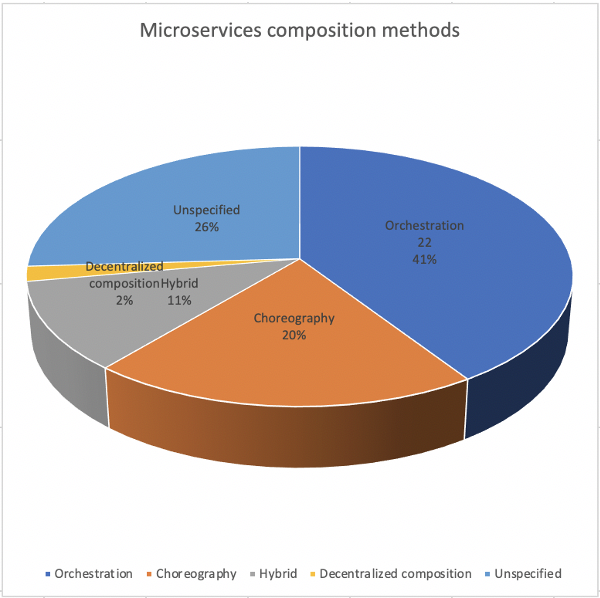
\includegraphics[scale=0.60]{mscompcore.png}}
  \caption{Microservices composition methods.}
  \label{fig}
\end{figure*}


\subsection{Microservices composition from the core composition perspective}


Figure 2 below shows that at 22\% of our studies, the model-based approach is the microservices composition method that is the most popular. This approach consists in modelling the entire microservices composition using existing modelling frameworks such as Business Process Modelling and Notation (BPMN) or UML which enables a diagrammatic representation of all the entities (microservices) and how they communicate (relationships) with each other as part of a composition process. The model approach is followed by a number of methods each representing between 5 and 10\% of our selected studies. These include the semantic annotation approach used in 8\% of the studies. The semantic annotation is technique that consist in using words to describe entities and provide linkages between them (Stork et al., 2019). S14 for instance describes how as part of a microservice composition process, a service description module extracts semantic information from a given service implementation to create a platform independent description for a service. The services could then be searched against specific annotations in their interfaces which represent a blueprint on how to interact with the service which developers can follow when building microservices. The container-based approach also accounts for 8\% of the selected studies and they are composition approaches that focuses on the implementation of microservices such as the one described in S13 which discuss an implementation approach for microservices composition based on docker container technology after outlining the steps of a proprietary algorithm for building microservices. The authors explain in S13 how 4 microservices A, B, C and D can be deployed independently in a docker container and communicate synchronously with one another to create an entire business process. Agent-based approaches accounts for 7\% of our selected studies. S7 is an example of agent-based approach. The authors discuss an automatic declarative and lightweight approach to semantically annotated microservices using agent-based clients. The main differentiator of this approach as noted by the authors is the ability to construct composition workflows dynamically by using the agents. This significantly reduces manual and costly effort involved in modelling workflows that cannot adapt to changes automatically 

Other microservices approaches are based on specific programming languages and generic or purposely designed algorithms which represent each 7\% of our selected studies. CSP\# is used in S6 to analyse the realisability of microservices choreography under synchronous and asynchronous communication. CSP\# is an extension of CSP (communicating sequential process), a language for describing the interactions of concurrent and distributed systems that integrates  high-level modelling properties with low-level codes to enable system verification. This approach consists in analysing and comparing two choreographies, and if they are behaviourally equivalent it indicates the realisability of the choreography otherwise it is deemed unrealisable. The advantage of this approach are 3 folds: 1) Ability to model asynchronous communication. 2) The ability to achieve asynchronous communication message buffering through its global variables. 3) Ability to model and simulate synchronous and asynchronous communication models through its integration to a PAT model checker.
S39 discusses choreography in Microservice Oriented Architecture (MOA) for Industry 4.0 using platform known as molecular,  an open-source development framework for MOA running on Node.js. The authors explain in S39 how applications can be created through two types of choreographies also referred to as internal and external applications. Internal applications are compatible with the molecular platform. The choreography of internal applications follows a predefined sequence and uses a messaging service known as the transporter. External applications on the contrary can be built on any platform, and their choreography is performed externally using REST communication through a gateway component while microservices communicate with one another through the transporter.
S47 is another language-based composition approach. Chimera Markup Language (CHIML) uses JSON-RPC for data exchange but does also support HTTP giving developers flexibility to create custom protocols. While their work focuses on improving some of the weaknesses of CHIML, the authors reference it as one of the languages of choice for microservices orchestration. Chimera has a central component known as Chimera core which is responsible for orchestrating external programs into a single process flow contained in a YAML chain file. There are two other components that make up the Chimera framework namely Chimera-Service and Chimera-Sender brings which are responsible for the HTTP helping make the entire framework distributed (Gunawan et al., 2017)
In S5 the authors provide a classification compositions approaches based on QoS (4\% of our selected studies) which they group into two categories: static and adaptative. The former makes use of Internal adaption techniques algorithms (e.g., Reinforcement learning, AI planning) to make composition decision. The latter uses Particle Swarn Optimization (PSO) and genetic algorithm. 
The Jolie (Java Orchestration Language Interpreter Engine) is introduced in S17. Jolie is a language that allows writing program from a data-driven instead of process-driven perspective. According to the authors of S17, Jolie is designed for workflow and service composition and is made of 4 concepts that make the language a good fit for microservice architecture. 1. Interfaces to provide a description of the functionalities and advertise the service. 2. Port to describe how the functionalities of a given microservice can be accessed on the network which is key for inter-service communication. 3. Workflows for implementing the service operations with all the required dependencies to define the order in which microservice execute and what are the triggers. 4. Processes which is a running instance of a workflow and as services interact with other services and clients there is a need to support concurrent execution. For that reason, processes run independently from each other which aligns with the self-contained characteristic of microservices. 6\% of the selected studies uses event-driven approach followed closely by DSL (Domain Specific Language) (5\%) and cloud- based approaches (5\%). S2 and S3 use a combination of DSL and event-driven approaches. S3 describes Beethoven as a lightweight event-driven for microservice composition that uses a textual DSL known as Partitur which helps create the workflow for the composition and uses its build-in Even-Condition-Action (ECA) even handling to coordinate the actions of the microservices as part of the composition workflow. Similarly, S2 also introduces Medley, a lightweight event-based platform for microservice composition. Medley uses DSL to define a workflow that defines how to assemble the service and the composition logic, which is then passed to a compiler that produces low-level code enabling the communication among the composite services. Medley maps services to process and each process has its input channel for listening to incoming events and an output channel for publishing outgoing events. S22 describes the composition of cloud native applications using a cloud orchestrator component that also manages the resources of each participating service. This approach uses modern cloud functionalities such as distributed in-memory key-value store to store the state” service functionalities and assign those functionalities cluster nodes using an internal algorithm. This helps implement cloud functionalities such as autoscaling, self-healing within atomic services as a stateless application component which provides the self-management capability. 
Contract-based, Transaction-based and Human interaction-based approaches represent 3\% each of our selected studies. In S44 the authors discuss an example of a contract-based approach for managing communication between services in their approach to typified microservice composition and discovery. A service contract here can be seen as a descriptor that contains information on how the service should be invoked, its address and it uses protocols such as OpenAPI or WSDL. Service collaboration is done synchronously (request-response) or asynchronously (event-driven). A contract is defined as sequence of message types in order to differentiate between to help level differences between method.  A HTTP call would be a chain of two messages whereas an event would be a single chain element. A contract also contains an endpoint of service which provides contract realisation (provider), an address to check the contract provider urgency - a direction of every chain unit - is the message incoming or outgoing for provider. User contract does not specify an interface though it has the same format as the provider, and it ensures that the system’s services have all dependencies and work correctly.
Human-collaboration approach is described in S10 and make use of collaborative modelling in the context of Microservice Architecture. The organisational structure  of microservices is divided into 2 separate scope of collaboration: the team internal scope which means a collaboration between team members to manage one or more microservices. The team external scope which is the inter-teams collaboration using services interfaces for the realisation of their service.The assembly of the services into an overall system are a form of team external collaboration. A model of the system is designed using UML and a single team is responsible for defining a model for the microservice that it is responsible for. To compose an overall system model, a central model registry is used and it is the registry that assembles the microservices using individual service interfaces and their dependencies to other services. To ensure a successful composition of the system model, each microservice model is tested at each release for its integrability.
The authors of S32 illustrates a transaction by showcasing an  e-commerce application example. When a microservice execute a transaction locally in an event based choreography, it publishes and an output event which can be picked up by another subscribing microservice which consumes that event to trigger the execution of this other microservice local transaction This process continues until the last microservice which does not publish an event (say because it needs to send a response back to a client request) and that will signify the end of the transaction. There are 7 other techniques for microservices composition from the perspective of the composition logic that are less popular as they represent each 2\% or less of our selected papers. These are: Labelled transition systems (LTS); an approach for choreography analysis which is described in S4. In this approach composite microservices are generated from a given choreography and using refinement checking the choreography is analysed for both synchronous and asynchronous composition and the composed service is compared against the specification to determine the validity of the composition.
An example of ML-based composition approach is described in S45, it performs a runtime search to identify behavior of microservices which machine learning can navigate at runtime and tailor the system to the current environment in order for the composed service to fulfill a given function. The authors explore what is the best to divide a human engineer and the machine self-learning. Microservices are put in a central folder and the machine then takes them to assemble them into composite service using its assembly module. 
API-based approach to microservices composition is described in S15 in the form of backend as a service (BaaS) platform which decompose an API into discrete services and integrate them into a microservice architecture. This is a 4-step process: 1. A design of a BaaS, 2. The functional requirements of the services are mapped to APIs which help produce API contracts. 3. Contracts are decomposed into microservices 4. Microservices are integrated for their consolidated execution. 
Interaction awareness approach is described in S20 as a framework for microservice deployment. In this approach each microservice is made of several instances which can be scheduled by a cloud provider in 4 steps: 1. Capture interactions between microservices and generate an interaction graph. Interactions can be captured by way of load test scripts.
2. Calculation of the interaction factor which is the number of interactions among microservices. 3. Derive scheduling strategies based on interaction factors. This is done by the scheduling engine. Microservices are then assigned to corresponding infrastructure components as well as making microservices discoverable by entering their components’ metadata in a central registry service. 
S11 discusses client-based collaboration as part of a Client-based MicroServices automatic collaboration (MSAC) framework that uses microservices instances at runtime and passed to the adjacent microservice to achieve dynamic collaboration of microservices. Process coordination is discussed in S31 with an illustration of how multiple coordination processes can be used in a decentralized fashion to coordinate large, distributed process structure. Micron-based approach to service composition is discussed in S16. Microns are standardized general-purpose processing commands that are suitable for building components and connectors. Microns accept inputs performs a given task and produces corresponding output. Each microns represent a microservice operation, and multiple microns can be grouped to form a composite microservice-system. 

\begin{figure*}[htbp]
 \centerline{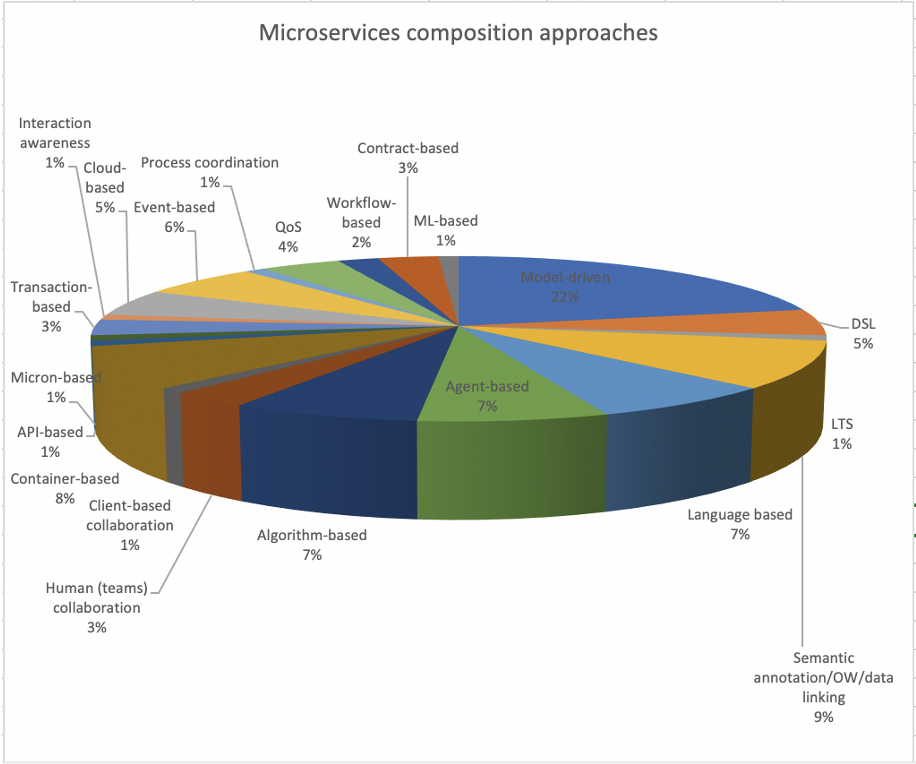
\includegraphics[scale=0.60]{mscomappr.png}}
  \caption{Microservices composition approaches.}
  \label{fig}
\end{figure*}

\textbf{RQ2:} Which frameworks are used to compose microservices?

Fig. 3 below shows that we have identified 33 frameworks from the selected studies of this SLR of which semantic annotation is the one that has the highest number of studies with 5 in total. The next framework to microservices composition that is most widely used according to our study, with 4 studies each are the Domain Specific Language (DSL) and the ad hoc approach that uses generic approach of building applications to achieve the composition of microservices as opposed to using purposely designed languages or platforms for service composition. Next, we had 6 frameworks in that were used in two studies each, these include BPMN, Jolie programming, DSML, MDE, Web framework and g-choreography. S25 discuss DSML which fosters model-centric developnent whereby each team uses a separate model repository for each microservice model. Such repository can then be integrated with domain-specific modeling languages (DSMLs) designed to address  a specialized viewpoint for microservice development. There are 3 viewpoints in total: the Data Viewpoint that holds concepts for specifying a microservice’s model details; the Service Viewpoint which guides the modeling of interfaces and dependencies to other teams’ services; tthe Operation Viewpoint for the modelling of deployment and operation of a service.
S29 present MDE and g-choreography as a workflow model that use global choreography which they refer to as a structured version of global graph. The global choreography defines the syntax for the exchange of information between microservices in a sequential, parallel or branching (fork) mode. 
S41 discuss an implementation of web framework of microservice composition based on Spring cloud which is based Java language and uses 
JNI as well as RPC for communication with microservices written in other languages such as C++, Python. Spring Cloud does provide the following capabilities that help provide a robust service composition: service discovery management, service fault tolerance, service gateway, and service configuration, load balancing, and messaging. The remaining frameworks are used in only one study. 

%\begin{figure*}[htbp]
\begin{figure*}[htb!]
 \centerline{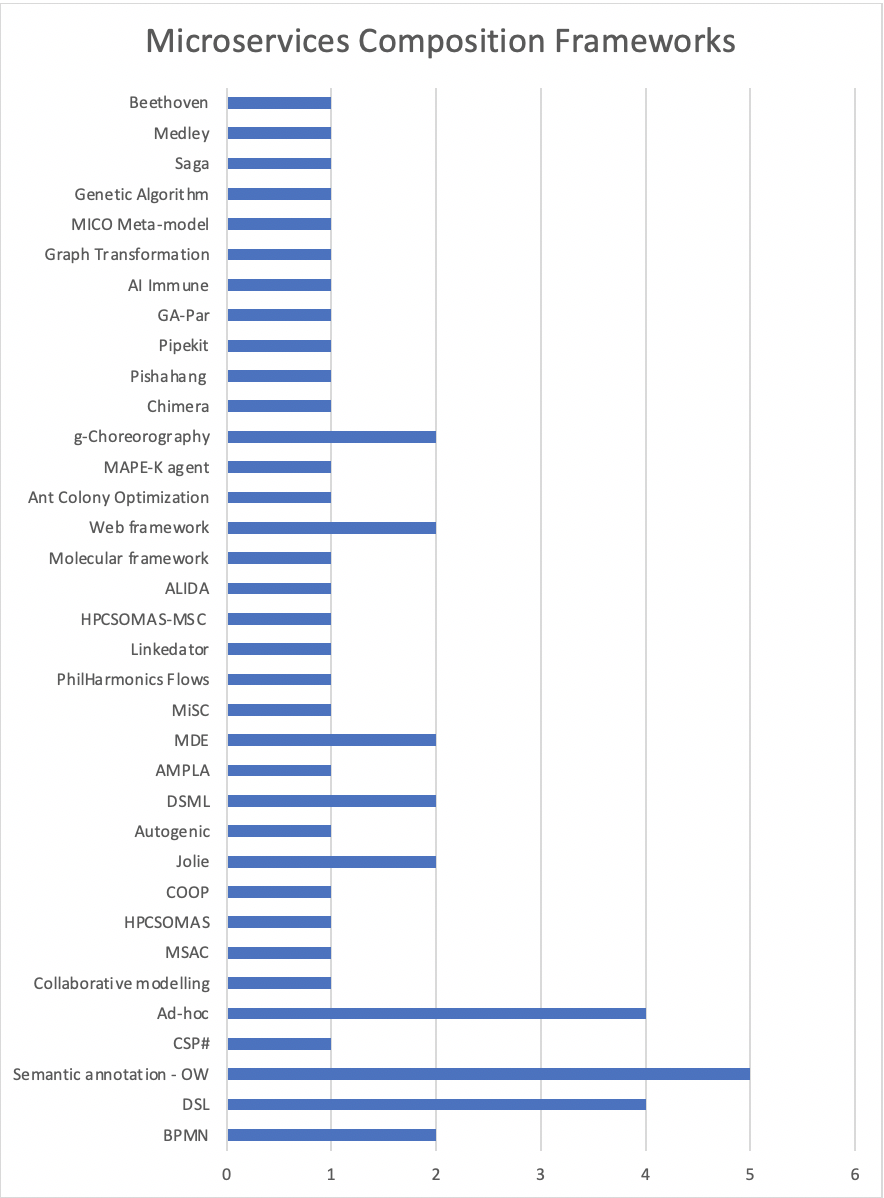
\includegraphics[scale=0.60]{mscompframw.png}}
  \caption{Microservices composition frameworks.}
  \label{fig}
\end{figure*}

\section{Results analysis and discussion}

This section discusses the SLR results in respect to our target RQs:

\begin{itemize}
\item{What are the curent approaches to microservices composition?}
\item{Which frameworks are used to compose microservices?}
\end{itemize}

Table 1 below shows the papers that discuss each of the identified microservice composition methods.

%\begin{table*}[]
\begin{table*}[ht!]
\begin{center}
\scriptsize
\begin{tabular}{ | m{20em} | m{20em} | }
\hline
\multicolumn{1}{|c|}{\textbf{Microservices composition approach}} & \multicolumn{1}{c|}{\textbf{Studies}}                                                                   \\ \hline
Model Driven                                                      & S1,   S6, S7, S8, S10, S11, S16, S24, S25, S26, S27, S28, S29, S31, S34, S35, S36,   S40, S46, S53, S55 \\ \hline
DSL                                                               & S2,   S43 S24, S72, S388                                                                                \\ \hline
LTS                                                               & S4                                                                                                      \\ \hline
Semantic   annotation/OW/data linking                             & S5,   S7, S8, S14, S33, S36, S42, S43, S54                                                              \\ \hline
Language   based                                                  & S6,   S17, S24, S28, S39, S41, S47                                                                      \\ \hline
Agent-based                                                       & S7,   S8, S9, S12, S21, S35, S43                                                                        \\ \hline
Algorithm-based                                                   & S5,   S7, S42, S50, S54, S55, S56                                                                       \\ \hline
Human   (teams) collaboration                                     & S10,   S23, S25                                                                                         \\ \hline
Client-based   collaboration                                      & S11                                                                                                     \\ \hline
Container-based                                                   & S13,   S18, S20, S21, S30, S23, S34, S49                                                                \\ \hline
API-based                                                         & S15                                                                                                     \\ \hline
Micron-based                                                      & S16                                                                                                     \\ \hline
Transaction-based                                                 & S19,   S32, S57                                                                                         \\ \hline
Interaction   awareness                                           & S20                                                                                                     \\ \hline
Cloud-based                                                       & S21,   S22, S30, S48, S134                                                                              \\ \hline
Event-based                                                       & S1,   S2, S3, S30, S94, S44                                                                             \\ \hline
Process   coordination                                            & S31                                                                                                     \\ \hline
QoS                                                               & S5,   S107, S42, S51                                                                                    \\ \hline
Workflow-based                                                    & S7,   S38                                                                                               \\ \hline
Contract-based                                                    & S15,   S44, S52                                                                                         \\ \hline
\end{tabular}
\end{center}
\caption{Microservices composition methods}
\label{table:1}
\end{table*}

While Table 2 below shows the identified composition frameworks and the papers in which they are used.

%\begin{table*}[]
\begin{table*}[ht!]
\begin{center}
\scriptsize
\begin{tabular}{ | m{20em} | m{20em} | }
\hline
\multicolumn{1}{|c|}{\textbf{Framework}}     & \multicolumn{1}{c|}{\textbf{Study   code}} \\ \hline
BPMN                                         & S1,   S7                                   \\ \hline
DSL                                          & S2,   S3, S24, S38                         \\ \hline
Semantic   annotation - OW                   & S3,   S5, S7, S8, S14                      \\ \hline
CSP\#                                        & S6                                         \\ \hline
Ad-hoc                                       & S9,   S13, S32, S34                        \\ \hline
Collaborative   modelling                    & S10                                        \\ \hline
MSAC (MicroServices Automatic Collaboration) & S11                                        \\ \hline
HPCSOMAS                                     & S12                                        \\ \hline
COOP                                         & S14                                        \\ \hline
Jolie                                        & S17,   S28                                 \\ \hline
Autogenic                                    & S18                                        \\ \hline
DSML (DS Modelling language)                 & S10,   S25                                 \\ \hline
AMPLA                                        & S27                                        \\ \hline
MDE                                          & S29,   S40                                 \\ \hline
MiSC                                         & S30                                        \\ \hline
PhilHarmonics   Flows                        & S31                                        \\ \hline
Linkedator                                   & S33                                        \\ \hline
HPCSOMAS-MSC                                 & S35                                        \\ \hline
ALIDA                                        & S36                                        \\ \hline
Molecular   framework                        & S39                                        \\ \hline
Web   framework                              & S41,   S45                                 \\ \hline
Ant   Colony Optimization                    & S42                                        \\ \hline
MAPE-K   agent                               & S43                                        \\ \hline
g-Choreorography                             & S29,   S40                                 \\ \hline
Chimera                                      & S47                                        \\ \hline
Pishahang                                    & S48                                        \\ \hline
Pipekit                                      & S49                                        \\ \hline
GA-Par                                       & S50                                        \\ \hline
AI   Immune                                  & S51                                        \\ \hline
Graph   Transformation                       & S53                                        \\ \hline
MICO   Meta-model                            & S55                                        \\ \hline
Genetic   Algorithm                          & S56                                        \\ \hline
Saga                                         & S57                                        \\ \hline
Medley                                       & S3                                         \\ \hline
Beethoven                                    & S2, S4                                     \\ \hline
\end{tabular}
\end{center}
\caption{Microservices composition frameworks}
\label{table:2}
\end{table*}

While ad-hoc approaches to microservices composition are still widely used, some of the studies such as S1 demonstrates that composing microservices using frameworks like BPMN are faster than ad hoc method and allow for easy and faster implementation of changes which makes it a good candidate for industry adoption which remains one of the biggest limitations of these frameworks. Only S3, S6 and S41 out of all the frameworks have a commercial implementation. Medley version used by practitioner is known as CProdirect. 
The fact that the highest number of frameworks use known technology such semantic annotation, DSL, labelled transition systems and widely use modelling language such as UML and BPMN as well as common protocols such as HTTP, JSON, WDSL, RPC as opposed to using proprietary or purposely designed for microservice composition, make the wide adoption through common standards an achievable task. Some of the composition methods and frameworks are made of a combination of methods and or other frameworks which allows some optimization by bringing together the strengths of individual methods. A good example is S5 that demonstrate the superior quality of a hybrid approach to service composition in terms of time effectiveness and resources consumption (memory and power).
Because most composition methods and frameworks are implemented using common technologies, they naturally inherit the strengths and the limitation of these underlying technologies. This is illustrated in S8 where the drawbacks of using an agent-based composition that add additional procession overhead approach are discussed while being providing capabilities such as off line activities by the agent in case of a disconnect with the central orchestrator component. This is a typical trade off of performance versus reliability between agent-based and agentless solution.
The results show that a significant number of frameworks are designed or tested for the cloud and containers which supports Dai et al. (2020) view that service composition as an growing area of interest for cloud computing.

\section{Related work}

In this section we present some of the systematic literature reviews (SLR) that have been done already for studies that focus on service composition. One of the most significant is that of Hayyolalam \& Kazem (2018)  who conducted a SLR in which they review papers that discuss QoS-aware approaches to service composition in a cloud environment. Customers expect a certain level of service quality from their service provider which is specified in the form of service level agreements (SLAs) that bind the two parties. Those SLAs are made of a number of KPIs which Hayyolalam et al. (2018) refer to as QoS attributes or QoS metrics. In their study, they concentrate specifically on the following attributes: cost, availability, response time, reliability, throughput, execution time and reputation of which cost, availability and response time are the most used by researchers according to their survey with an average of 16\% out the 50 papers that were in scope of their studies. Hayyolalam \& Pourhaji Kazem (2018) also classify papers on one had based on the service composition environment as well as and whether the study is conducted on a single or multi-cloud, and on the other based on whether is single or multi-objective optimization. Their survey uncover a pattern in which service composition in a cloud environment is described ‘as a single-objective problem with local/global QoS optimization or a multi-objective problem with global QoS optimization’ (Hayyolalam \& Pourhaji Kazem, 2018). One of the limitations of this survey is that it does not focus on how the actual service composition is done nor does it inform the reader on what frameworks are used in the service composition process. 

Another notable SLR on cloud service composition is that of Vakili \& Navimipour (2017) who view service composition as a new way of integrating multiple individual services in the cloud order to fulfill complex user requirements. Their study focus on identifying the challenges associated service composition in the cloud environment as well as the current approaches for service composition and service selection and the underlying activities that are involved in the on the-fly integration of cloud services as they are provisioned to help address complex end-users requests. Vakili \& Navimipour (2017) start by acknowledging the efforts that. Have been done in providing frameworks (platforms and languages) for web service composition which they classify into three main categories which include: workflow-based approaches; XML-based approaches (e.g. BPEL4WS) and ontology-based approaches (e.g. OWL-S and DAML-S). The authors uncovered from their study, three main cloud service composition techniques including the framework-based, heuristic-based and agent-based technique. One of the selected papers for this study is from Zhang et al. (2014) who proposed an example of framework-based technique based on a model generated from a solution algorithm that analyzes the characteristics of services resources in cloud manufacturing.

An example of agent-based service composition technique is proposed by Wang et al., 2016a, Wang et al., 2016b and the method uses a multi-agent reinforcement learning algorithm to interact with the environment in real time in order to generate an optimal composition strategy on the fly.
In Karimi et al. (2016), the authors discuss an example of heuristic-based technique for which the service composition is done based on the SLA contract in the cloud environment. The researchers use data mining techniques in service composition and genetic algorithm to ensure a quality service is provided as fast as possible to end-users thereby helping ensure SLA compliance. Vakili \& Navimipour (2017) survey shows that efficiency, optimization and time are the QoS metrics that are the most widely used in comparison to scalability and cost.

The fast adoption of cloud computing and the growing number of cloud services has made it impossible for a single service to address the variety of (complex) use cases from multiple cloud services consumers. For that reason, Jula et al. (2014) recognize the need to have a service composition module embedded within a cloud environment in order to bring together a set of atomic services in order to provide a complex functionality. The authors in Jula et al. (2014) consider that a composite service is made of n number of unique services (USs) with p number of QoS parameters. To that end, service composition constitutes a workflow made of a sequence of unique services. Their study identified five categories of service composition approaches which are: classic and graph-based algorithms (CGBAs), combinatorial algorithms (CAs), machine-based approaches (MBAs), structures (STs), and frameworks (FWs) (Jula et al., 2014).

Ye, Zhou, \& Bouguettaya (2011) cited in Amin et al. (2014) demonstrate that the combinatorial algorithm for instance uses QoS parameters which is divides into equal, ascending and descending groups and normalise their values by way of additive weighting, which generates a new model that computes the Q0S of composite service is proposed. Similarly, the machine-based method as described by Amin et al. (2014) selects the path for composite services with highest QoS based on a two-phase process. First it creates a service tree and a target process discarding any improper paths in the tree by applying a policy which also helps reduce processing time. The second phase is about selection the most optimal path which corresponds to QoS parameters that best match the user requirements. 

\section{Conclusion \& future work}

In this research, we present a SLR on microservices composition, we selected 59 papers after rigorously applying our defined inclusion and exclusion criteria, which we reviewed thoroughly and extracted data relevant to our 2 research questions. We looked at microservices composition methods from two perspectives: 1. How the composition is managed and 2. The core composition logic. For the former, the orchestration method is the most used in research focused on microservices composition with 41\% of our selected papers. For the latter, 20\% of the selected papers for our study use choreography as a composition method, while 11\% use both methods (orchestration and choreography) which is classified as hybrid. The former (core composition logic perspective) is more diversified with a total of 20 methods used in our selected papers of which the modelling approach is the most popular with 22\% of our selected papers using this method, followed by the semantic annotation and container-based with each representing 8\% of the selected papers. Some the least used methods (2\% or less of the selected papers) include ML, API and microns-based composition methods. We also find out through this research that 34 frameworks specifically designed for composing microservices in the selected studies some of which include Medley, Beethoven, BPMN, Saga, CSP\# and Jolie. Our study shows that microservices-based systems are still built using an ad-hoc approach which is proportionally higher than 50\% of existing frameworks. Furthermore, the vast majority of existing frameworks are yet to be adopted in the industry with only 3 (Medley, CSP\# and Web framework) out of the 34 of selected papers having a commercial version.
While some of the benefits of microservices composition techniques were highlighted in this study, a much deeper research which compares and contrasts the different techniques would be beneficial in that it would aid practitioners in making a decision on which approach to choose given a set of requirements. Furthermore, a follow up study that focuses in identifying blockers for industry adoption of existing frameworks maybe useful. From our perspective, we will be looking to further this study with the design of a novel approach for composing microservices which may be a combination of the strengths of the ones identified in this research and a solution to some or all of their pitfalls.

\end{multicols}
\pagebreak 
\section{References}

\begin{enumerate}

\item Vahideh Hayyolalam, Ali Asghar Pourhaji Kazem, A systematic literature review on QoS-aware service composition and selection in cloud environment, Journal of Network and Computer Applications, Volume 110, 2018, Pages 52-74



\item Asrin Vakili, Nima Jafari Navimipour, Comprehensive and systematic review of the service composition mechanisms in the cloud environments, Journal of Network and Computer Applications, Volume 81, 2017, Pages 24-36

\item Amin Jula, Elankovan Sundararajan, Zalinda Othman, Cloud computing service composition: A systematic literature review, Expert Systems with Applications, Volume 41, Issue 8, 2014,
Pages 3809-3824

\item Baresi L., Garriga M. (2020) Microservices: The Evolution and Extinction of Web Services?. In: Bucchiarone A. et al. (eds) Microservices. Springer

\item Peishi Jiang, Mostafa Elag, Praveen Kumar, Scott Dale Peckham, Luigi Marini, Liu Rui,
A service-oriented architecture for coupling web service models using the Basic Model Interface (BMI), Environmental Modelling \& Software, Volume 92, 2017, Pages 107-118

\item Lagares Lemos, Angel \& Daniel, Florian \& Benatallah, Boualem. (2015). Web Service Composition. ACM Computing Surveys. 48. 1-41. 10.1145/2831270

\item Claro, Daniela \& Albers, Patrick \& Hao, Jin-Kao. (2006). Web Services Composition. 

\item Garriga M. (2018) Towards a Taxonomy of Microservices Architectures. In: Cerone A., Roveri M. (eds) Software Engineering and Formal Methods. SEFM 2017. Lecture Notes in Computer Science, vol 10729. Springer, Cham

\item Dmitry Namiot, Manfred Sneps-Sneppe (2014). On Micro-services Architecture. International Journal of Open Information Technologies ISSN: 2307-8162 vol. 2, no.9, 2014

\item Singleton, A. (2016). The Economics of Microservices. IEEE Cloud Computing,3(5), 16-20

\item Chen, L. (2018). Microservices: Architecting for Continuous Delivery and DevOps. 2018 IEEE International Conference on Software Architecture (ICSA). 

\item C. Jatoth, G. R. Gangadharan and R. Buyya, "Computational Intelligence Based QoS-Aware Web Service Composition: A Systematic Literature Review," in IEEE Transactions on Services Computing, vol. 10, no. 3, pp. 475-492, 1 May-June 2017

\item M.S. Hamzehloui, S. Sahibuddin, A. Ashabi, A study on the most prominent areas of research in microservices. Int J Mach LearnComput, 9 (2) (2019), pp. 242-247

\item B. Kitchenham and S. Charters, "Guidelines for performing systematic literature reviews in software engineering", 2007

\item P. Jamshidi, C. Pahl, N. C. Mendonça, J. Lewis and S. Tilkov, "Microservices: The Journey So Far and Challenges Ahead," in IEEE Software, vol. 35, no. 3, pp. 24-35, May/June 2018

\item Valderas, P., Torres, V. and Pelechano, V., 2020. A microservice composition approach based on the choreography of BPMN fragments. Information and Software Technology, 127, p.106370.

\item Monteiro D., Gadelha R., Maia P.H.M., Rocha L.S., Mendonça N.C. (2018) Beethoven: An Event-Driven Lightweight Platform for Microservice Orchestration. In: Cuesta C., Garlan D., Pérez J. (eds) Software Architecture. ECSA 2018. Lecture Notes in Computer Science, vol 11048. Springer, Cham.

\item Ben Hadj Yahia E., Réveillère L., Bromberg YD., Chevalier R., Cadot A. (2016) Medley: An Event-Driven Lightweight Platform for Service Composition. In: Bozzon A., Cudre-Maroux P., Pautasso C. (eds) Web Engineering. ICWE 2016. Lecture Notes in Computer Science, vol 9671. Springer, Cham.

\item F. Dai, Q. Mo, Z. Qiang, B. Huang, W. Kou and H. Yang, "A Choreography Analysis Approach for Microservice Composition in Cyber-Physical-Social Systems," in IEEE Access, vol. 8, pp. 53215-53222, 2020

\item Singhal, N. and Sakthivel, U., 2019. Efficient Hybrid Research for QoS-Aware Microservice Composition. International Journal of Recent Technology and Engineering, 8(2), pp.5251-5255.

\item R. Wu, Q. Duan, F. Dai, H. Yang, Y. Zhang and B. Xie, "Research on the Realizability of Microservice Interaction Contract Based on CSP\#," 2019 IEEE 43rd Annual Computer Software and Applications Conference (COMPSAC), Milwaukee, WI, USA, 2019, pp. 622-627

\item Oberhauser, R. and Stigler, S. (2017). Microflows: Enabling Agile Business Process Modeling to Orchestrate Semantically-Annotated Microservices.In Proceedings of the Seventh International Symposium on Business Modeling and Software Design - Volume 1: BMSD, ISBN 978-989-758-238-7, pages 19-28.

\item Salvadori, I., \& Huf, A. (2016). Agent Based Composition Model - ICWI 2016 [Data set]. figshare.

\item Singhal, N., Sakthivel, U., \& Raj, P. (2019). Selection Mechanism of Micro-Services Orchestration Vs. Choreography. International Journal of Web \& Semantic Technology (IJWesT), 10(1), 25.

\item Sorgalla J., Rademacher F., Sachweh S., Zündorf A. (2018) On Collaborative Model-Driven Development of Microservices. In: Mazzara M., Ober I., Salaün G. (eds) Software Technologies: Applications and Foundations. STAF 2018. Lecture Notes in Computer Science, vol 11176. Springer, Cham.

\item Wang R, Chen S Z, Feng Z Y, et al. A client microservices automatic collaboration framework based on fine-grained app. In: Proceedings of 2018 IEEE International Conference on Services Computing (SCC), 2018. 25–32

\item Oparin, G. A., Bogdanova, V. G., \& Pashinin, A. A. (2020). Automated tools for the development of microservice compositions for hybrid scientific computations. CEUR Workshop Proceedings, 2638, 201–213. 

\item Ke, J., Xu, J. B., \& Feng, S. (2019). An Implementation of Service Composition for Enterprise Business Processes. IOP Conference Series: Earth and Environmental Science, 234(1). 

\item Groh, O., Baraki, H., Jahl, A., \& Geihs, K. (2019). COOP - automatiC validatiOn of evOlving microservice comPositions. CEUR Workshop Proceedings, 2510. 

\item Dudjak, Mario \& Martinovic, Goran. (2020). An API-first methodology for designing a microservice-based Backend as a Service platform. Information technology and control. 49. 206-223.

\item S. Rasmy, "Microns: Commands for Building Bubble Microservices," 2018 Sixth International Conference on Enterprise Systems (ES), Limassol, Cyprus, 2018, pp. 158-165,

\item Bucchiarone, Antonio \& Dragoni, Nicola \& Dustdar, Schahram \& Lago, Patricia \& Mazzara, Manuel \& Rivera, Victor \& Sadovykh, Andrey. (2019). Microservices: Science and Engineering. 

\item Kehrer, Stefan \& Blochinger, Wolfgang. (2018). AUTOGENIC: Automated Generation of Self-configuring Microservices. 35-46.

\item Xue, G., Deng, S., Liu, D., \& Yan, Z. (2021). Reaching consensus in decentralized coordination of distributed microservices. Computer Networks, 187.

\item Joseph, C. T., \& Chandrasekaran, K. (2020). IntMA: Dynamic Interaction-aware resource allocation for containerized microservices in cloud environments. Journal of Systems Architecture, 111.

\item Tapia, F., Mora, M. A., Fuertes, W., Aules, H., Flores, E., \& Toulkeridis, T. (2020). From monolithic systems to microservices: A comparative study of performance. Applied Sciences (Switzerland), 10(17). 

\item Toffetti, G., Brunner, S., Blöchlinger, M., Spillner, J., \& Bohnert, T. M. (2017). Self-managing cloud-native applications: Design, implementation, and experience. Future Generation Computer Systems, 72, 165–179. 

\item Schäffer, E., Mayr, A., Fuchs, J., Sjarov, M., Vorndran, J., \& Franke, J. (2020). Microservice-based architecture for engineering tools enabling a collaborative multi-user configuration of robot-based automation solutions. Procedia CIRP, 86, 86–91.

\item Monteiro, D., Maia, P. H. M., Rocha, L. S., \& Mendonça, N. C. (2020). Building orchestrated microservice systems using declarative business processes. Service Oriented Computing and Applications, 14(4), 243–268.

\item Sorgalla, J., Rademacher, F., Sachweh, S., \& Zündorf, A. (2018). On collaborative model-driven development of microservices. Lecture Notes in Computer Science (Including Subseries Lecture Notes in Artificial Intelligence and Lecture Notes in Bioinformatics), 11176 LNCS, 596–603.

\item Santos, N., Rodrigues, H., Ferreira, N., \& Machado, R. J. (2019). Inputs from a Model-Based Approach Towards the Specification of Microservices Logical Architectures: An Experience Report. Lecture Notes in Computer Science (Including Subseries Lecture Notes in Artificial Intelligence and Lecture Notes in Bioinformatics), 11915 LNCS, 473–488.

\item Bravetti, M., Giallorenzo, S., Mauro, J., Talevi, I., \& Zavattaro, G. (2019). Optimal and automated deployment for microservices. Lecture Notes in Computer Science (Including Subseries Lecture Notes in Artificial Intelligence and Lecture Notes in Bioinformatics), 11424 LNCS, 351–368

\item Yussupov, V., Breitenbucher, U., Krieger, C., Leymann, F., Soldani, J., \& Wurster, M. (2020). Pattern-based Modelling, Integration, and Deployment of Microservice Architectures. Proceedings - 2020 IEEE 24th International Enterprise Distributed Object Computing Conference, EDOC 2020, 40–50

\item Xue, G., Deng, S., Liu, D., \& Yan, Z. (2021). Reaching consensus in decentralized coordination of distributed microservices. Computer Networks, 187.

\item G. F. Gunawan, M. Amien and J. F. Palandi, "Chimera — Simple language agnostic framework for stand alone and distributed computing," 2017 4th International Conference on Computer Applications and Information Processing Technology (CAIPT), Kuta Bali, Indonesia, 2017, pp. 1-10

\item Bucchiarone, A., Soysal, K., \& Guidi, C. (2020). A Model-Driven Approach Towards Automatic Migration to Microservices. Lecture Notes in Computer Science (Including Subseries Lecture Notes in Artificial Intelligence and Lecture Notes in Bioinformatics), 12055 LNCS, 15–36.

\item Coto, A., Guanciale, R., \& Tuosto, E. (2020). Choreographic development of message-passing applications: a tutorial. Lecture Notes in Computer Science (Including Subseries Lecture Notes in Artificial Intelligence and Lecture Notes in Bioinformatics), 12134 LNCS, 20–36.

\item Nordli, E. T., Nguyen, P. H., Chauvel, F., \& Song, H. (2020). Event-based customization of multi-tenant saas using microservices. Lecture Notes in Computer Science (Including Subseries Lecture Notes in Artificial Intelligence and Lecture Notes in Bioinformatics), 12134 LNCS, 171–180.

\item Steinau, S., Andrews, K., \& Reichert, M. (2020). Coordinating large distributed relational process structures. Software and Systems Modeling.

\item Rudrabhatla, C. K. (2018). Comparison of event choreography and orchestration techniques in Microservice Architecture. International Journal of Advanced Computer Science and Applications, 9(8), 18–22.

\item Salvadori, I. L., Huf, A., Oliveira, B. C. N., Dos Santos Mello, R., \& Siqueira, F. (2017). Improving entity linking with ontology alignment for Semantic microservices composition. International Journal of Web Information Systems, 13(3), 302–323.

\item Park, J., Kim, D., \& Yeom, K. (2020). An Approach for Reconstructing Applications to Develop Container-Based Microservices. Mobile Information Systems, 2020.

\item Oparin, G. A., Bogdanova, V. G., \& Pashinin, A. A. (2020). Automated tools for the development of microservice compositions for hybrid scientific computations. CEUR Workshop Proceedings, 2638, 201–213

\item Profeta, D., Masi, N., Messina, D., Dalle Carbonare, D., Bonura, S., \& Morreale, V. (2019). A Novel Micro-Service Based Platform for Composition, Deployment and Execution of BDA Applications. Proceedings - 45th Euromicro Conference on Software Engineering and Advanced Applications, SEAA 2019, 182–185.

\item Singhal, N., Sakthivel, U., \& Raj, P. (2019). Efficient hybrid research for QoS-aware microservice composition. International Journal of Recent Technology and Engineering, 8(2), 5251–5255.

\item Song, Z., \& Tilevich, E. (2019). Equivalence-enhanced microservice workflow orchestration to efficiently increase reliability. Proceedings - 2019 IEEE International Conference on Web Services, ICWS 2019 - Part of the 2019 IEEE World Congress on Services, 426–433.

\item Bigheti, J. A., Fernandes, M. M., \& Godoy, E. D. P. (2019). Control as a Service: A Microservice Approach to Industry 4.0. 2019 IEEE International Workshop on Metrology for Industry 4.0 and IoT, MetroInd 4.0 and IoT 2019 - Proceedings, 438–443.

\item Rademacher, F., Sorgalla, J., Sachweh, S., \& Zundorf, A. (2019). Viewpoint-specific model-driven microservice development with interlinked modeling languages. Proceedings - 13th IEEE International Conference on Service-Oriented System Engineering, SOSE 2019, 10th International Workshop on Joint Cloud Computing, JCC 2019 and 2019 IEEE International Workshop on Cloud Computing in Robotic Systems, CCRS 2019, 57–66.

\item Ke, J., Xu, J. B., \& Feng, S. (2019). An Implementation of Service Composition for Enterprise Business Processes. IOP Conference Series: Earth and Environmental Science, 234(1)

\item Essayah, A., Youssfi, M., Bouattane, O., Mansouri, K., \& Illoussamen, E. (2019). QoS-based semantic micro services discovery and composition using ACO algorithm: Case study: E-learning platform. International Journal of Advanced Computer Science and Applications, 10(6), 159–168.

\item Dai, W., Wang, P., Sun, W., Wu, X., Zhang, H., Vyatkin, V., \& Yang, G. (2019). Semantic Integration of Plug-and-Play Software Components for Industrial Edges Based on Microservices. IEEE Access, 7, 125882–125892.

\item Gerasimov, N. (2019). New approach to typified microservice composition and discovery. Journal of Automation, Mobile Robotics and Intelligent Systems, 13(1), 79–83.

\item Filho, R. R., Desá, M. P., Porter, B., \& Costa, F. M. (2018). Towards Emergent Microservices for Client-Tailored Design. ARM 2018 - Proceedings of the 2018 Middleware, 7–12.

\item Hallal, R., Jaber, M., \& Abdallah, R. (2018). From Global Choreography to Efficient Distributed Implementation. Proceedings - 2018 International Conference on High Performance Computing and Simulation, HPCS 2018, 756–763

\item Gunawan, G. F., Palandi, J. F., \& Subari. (2018). Redesigning CHIML: Orchestration language for chimera- framework. Proceedings of the 3rd International Conference on Informatics and Computing, ICIC 2018

\item Kouchaksaraei, H. R., Dierich, T., \& Karl, H. (2018). Pishahang: Joint Orchestration of Network Function Chains and Distributed Cloud Applications. 2018 4th IEEE Conference on Network Softwarization and Workshops, NetSoft 2018, 308–312.

\item Chico De Guzman, P., Gorostiaga, F., \& Sanchez, C. (2018). Pipekit: A Deployment Tool with Advanced Scheduling and Inter-Service Communication for Multi-Tier Applications. Proceedings - 2018 IEEE International Conference on Web Services, ICWS 2018 - Part of the 2018 IEEE World Congress on Services, 379–382.

\item Wen, Z., Lin, T., Yang, R., Ji, S., Ranjan, R., Romanovsky, A., Lin, C., \& Xu, J. (2020). GA-Par: Dependable Microservice Orchestration Framework for Geo-Distributed Clouds. IEEE Transactions on Parallel and Distributed Systems, 31(1), 129–143.

\item Gao, M., Chen, M., Liu, A., Ip, W. H., \& Yung, K. L. (2020). Optimization of Microservice Composition Based on Artificial Immune Algorithm Considering Fuzziness and User Preference. IEEE Access, 8, 26385–26404.

\item Ardagna, C. A., Anisetti, M., Carminati, B., Damiani, E., Ferrari, E., \& Rondanini, C. (2020). A blockchain-based trustworthy certification process for composite services. Proceedings - 2020 IEEE 13th International Conference on Services Computing, SCC 2020, 422–429.

\item Bachras, M., \& Kontogiannis, K. (2020). Goal Modelling Meets Service Choreography: A Graph Transformation Approach. Proceedings - 2020 IEEE 24th International Enterprise Distributed Object Computing Conference, EDOC 2020, 30–39.

\item Jaber, M., Falcone, Y., Attie, P., Khalil, A.-A., Hallal, R., \& El-Hokayem, A. (2020). From global choreographies to verifiable efficient distributed implementations. Journal of Logical and Algebraic Methods in Programming, 115.

\item Lei, C., \& Dai, H. (2020). A Heuristic Services Binding Algorithm to Improve Fault-Tolerance in Microservice based Edge Computing Architecture. Proceedings - 2020 IEEE World Congress on Services, SERVICES 2020, 83–88

\end{enumerate}

\pagebreak

%\appendix
\begin{appendices}
\begin{table*}
\begin{center}
\scriptsize
\begin{tabular}{ | m{20em} | m{1cm}| m{20em} | m{1cm} | }
\hline
\textbf{Papers}                                                                                                                                                                                                                                                                                                                         & \textbf{Codes} & \textbf{Papers}                                                                                                                                                                                                                                                                                                                                                                                                              & \textbf{Codes}  \\ 
\hline
\textcolor[rgb]{0.2,0.2,0.2}{Valderas, P., Torres, V. and Pelechano, V., 2020. A microservice composition approach \ based on the choreography of BPMN fragments. ~Information and Software Technology, 127, p.106370.}                                                                                                                                                           & {S1}             & Bucchiarone, A., Soysal, K.,  Guidi, C. (2020). A Model-Driven Approach Towards Automatic Migration to Microservices. Lecture Notes in Computer Science (Including Subseries Lecture Notes in Artificial Intelligence and  Lecture Notes in Bioinformatics), 12055 LNCS, 15–36.                                                                                                                                                 & S28           \\ 
\hline

\textcolor[rgb]{0.2,0.2,0.2}{Monteiro D., Gadelha R., Maia P.H.M., Rocha L.S., Mendonça N.C. (2018) Beethoven: An Event-Driven Lightweight Platform for Microservice Orchestration. In: Cuesta C., Garlan D., Pérez J. (eds) Software Architecture. ECSA 2018. Lecture Notes in Computer Science, vol 11048. Springer, Cham.}                             & S2             & Coto, A., Guanciale, R.,  Tuosto, E. (2020). Choreographic development of message-passing applications: a tutorial. Lecture Notes in Computer Science (Including Subseries Lecture Notes in Artificial Intelligence and Lecture Notes in Bioinformatics), 12134 LNCS, 20–36.                                                                                                                                                   & S29             \\ 
\hline
\textcolor[rgb]{0.2,0.2,0.2}{Ben Hadj Yahia E., Réveillère L., Bromberg YD., Chevalier R., Cadot A. (2016) Medley: An Event-Driven Lightweight Platform for Service Composition. In: Bozzon A., Cudre-Maroux P., Pautasso C. (eds) Web Engineering. ICWE 2016. Lecture Notes in Computer Science, vol 9671. Springer, Cham.}                              & S3             & Nordli, E. T., Nguyen, P. H., Chauvel, F.,  Song, H. (2020). Event-based customization of multi-tenant saas using microservices. Lecture Notes in Computer Science (Including Subseries Lecture Notes in Artificial Intelligence and Lecture Notes in Bioinformatics), 12134 LNCS, 171–180.                                                                                                                                    & S30             \\ 
\hline
\textcolor[rgb]{0.2,0.2,0.2}{F. Dai, Q. Mo, Z. Qiang, B. Huang, W. Kou and H. Yang, "A Choreography Analysis Approach for Microservice Composition in Cyber-Physical-Social Systems," in~}\textcolor[rgb]{0.2,0.2,0.2}{IEEE Access}\textcolor[rgb]{0.2,0.2,0.2}{, vol. 8, pp. 53215-53222, 2020}                                                          & S4             & Steinau, S., Andrews, K.,  Reichert, M. (2020). Coordinating large distributed relational process structures. Software and Systems Modeling.                                                                                                                                                                                                                                                                                   & S31             \\ 
\hline
Singhal, N. and Sakthivel, U., 2019. Efficient Hybrid Research for QoS-Aware Microservice Composition.~\textit{International Journal of Recent Technology and Engineering}, 8(2), pp.5251-5255.                                                                                                                                                           & S5             & Rudrabhatla, C. K. (2018). Comparison of event choreography and orchestration techniques in Microservice Architecture. International Journal of Advanced Computer Science and Applications, 9(8), 18–22.                                                                                                                                                                                                                       & S32             \\ 
\hline
\textcolor[rgb]{0.2,0.2,0.2}{R. Wu, Q. Duan, F. Dai, H. Yang, Y. Zhang and B. Xie, "Research on the Realizability of Microservice Interaction Contract Based on CSP\#,"~}\textcolor[rgb]{0.2,0.2,0.2}{2019 IEEE 43rd Annual Computer Software and Applications Conference (COMPSAC)}\textcolor[rgb]{0.2,0.2,0.2}{, Milwaukee, WI, USA, 2019, pp. 622-627} & S6             & Salvadori, I. L., Huf, A., Oliveira, B. C. N., Dos Santos Mello, R.,  Siqueira, F. (2017). Improving entity linking with ontology alignment for Semantic microservices composition. International Journal of Web Information Systems, 13(3), 302–323.                                                                                                                                                                          & S33             \\ 
\hline
\textcolor[rgb]{0.333,0.333,0.333}{Oberhauser, R. and Stigler, S. (2017). Microflows: Enabling Agile Business Process Modeling to Orchestrate Semantically-Annotated Microservices.In Proceedings of the Seventh International Symposium on Business Modeling and Software Design - Volume 1: BMSD, ISBN 978-989-758-238-7, pages 19-28.}                 & S7             & Park, J., Kim, D.,  Yeom, K. (2020). An Approach for Reconstructing Applications to Develop Container-Based Microservices. Mobile Information Systems, 2020.                                                                                                                                                                                                                                                                   & S34             \\ 
\hline
Salvadori, I., \& Huf, A. (2016).~\textit{Agent Based Composition Model - ICWI 2016}~[Data set]. figshare.                                                                                                                                                                                                                                                & S8             & Oparin, G. A., Bogdanova, V. G.,  Pashinin, A. A. (2020). Automated tools for the development of microservice compositions for hybrid scientific computations. CEUR Workshop Proceedings, 2638, 201–213                                                                                                                                                                                                                        & S35             \\ 
\hline
Singhal, N., Sakthivel, U.,  Raj, P. (2019). Selection Mechanism of Micro-Services Orchestration Vs. Choreography. International Journal of Web  Semantic Technology (IJWesT), 10(1), 25.                                                                                                                                                                 & S9             & Profeta, D., Masi, N., Messina, D., Dalle Carbonare, D., Bonura, S.,  Morreale, V. (2019). A Novel Micro-Service Based Platform for Composition, Deployment and Execution of BDA Applications. Proceedings - 45th Euromicro Conference on Software Engineering and Advanced Applications, SEAA 2019, 182–185.                                                                                                                  & S36             \\ 
\hline
\textcolor[rgb]{0.2,0.2,0.2}{Sorgalla J., Rademacher F., Sachweh S., Zündorf A. (2018) On Collaborative Model-Driven Development of Microservices. In: Mazzara M., Ober I., Salaün G. (eds) Software Technologies: Applications and Foundations. STAF 2018. Lecture Notes in Computer Science, vol 11176. Springer, Cham.}                                & S10            & Singhal, N., Sakthivel, U.,  Raj, P. (2019). Efficient hybrid research for QoS-aware microservice composition. International Journal of Recent Technology and Engineering, 8(2), 5251–5255.                                                                                                                                                                                                                                    & S37             \\ 
\hline
\textcolor[rgb]{0.2,0.2,0.2}{Wang R, Chen S Z, Feng Z Y, et al. A client microservices automatic collaboration framework based on fine-grained app. In: Proceedings of 2018 IEEE International Conference on Services Computing (SCC), 2018. 25–32}                                                                                                       & S11            & Song, Z.,  Tilevich, E. (2019). Equivalence-enhanced microservice workflow orchestration to efficiently increase reliability. Proceedings - 2019 IEEE International Conference on Web Services, ICWS 2019 - Part of the 2019 IEEE World Congress on Services, 426–433.                                                                                                                                                         & S38             \\ 
\hline
Oparin, G. A., Bogdanova, V. G., \& Pashinin, A. A. (2020). Automated tools for the development of microservice compositions for hybrid scientific computations. \textit{CEUR Workshop Proceedings}, \textit{2638}, 201–213.~                                                                                                                             & S12            & Bigheti, J. A., Fernandes, M. M.,  Godoy, E. D. P. (2019). Control as a Service: A Microservice Approach to Industry 4.0. 2019 IEEE International Workshop on Metrology for Industry 4.0 and IoT, MetroInd 4.0 and IoT 2019 - Proceedings, 438–443.                                                                                                                                                                            & S39             \\ 
\hline
\end{tabular}
\end{center}
\end{table*}

\newpage

\begin{table*}
\begin{center}
\scriptsize
\begin{tabular}{ | m{20em} | m{1cm}| m{20em} | m{1cm} | }
\hline
Ke, J., Xu, J. B., \& Feng, S. (2019). An Implementation of Service Composition for Enterprise Business Processes. \textit{IOP Conference Series: Earth and Environmental Science}, \textit{234}(1).~                                                                                                                                                     & S13            & Rademacher, F., Sorgalla, J., Sachweh, S.,  Zundorf, A. (2019). Viewpoint-specific model-driven microservice development with interlinked modeling languages. Proceedings - 13th IEEE International Conference on Service-Oriented System Engineering, SOSE 2019, 10th International Workshop on Joint Cloud Computing, JCC 2019 and 2019 IEEE International Workshop on Cloud Computing in Robotic Systems, CCRS 2019, 57–66. & S40             \\ 
\hline
Groh, O., Baraki, H., Jahl, A., \& Geihs, K. (2019). COOP - automatiC validatiOn of evOlving microservice comPositions. \textit{CEUR Workshop Proceedings}, \textit{2510}.~                                                                                                                                                                               & S14            & Ke, J., Xu, J. B.,  Feng, S. (2019). An Implementation of Service Composition for Enterprise Business Processes. IOP Conference Series: Earth and Environmental Science, 234(1)                                                                                                                                                                                                                                                & S41             \\ 
\hline
\textcolor[rgb]{0.102,0.102,0.102}{Dudjak, Mario \& Martinovic, Goran. (2020). An API-first methodology for designing a microservice-based Backend as a Service platform. Information technology and control. 49. 206-223.}                                                                                                                               & S15            & Essayah, A., Youssfi, M., Bouattane, O., Mansouri, K.,  Illoussamen, E. (2019). QoS-based semantic micro services discovery and composition using ACO algorithm: Case study: E-learning platform. International Journal of Advanced Computer Science and Applications, 10(6), 159–168.                                                                                                                                         & S42             \\ 
\hline
\textcolor[rgb]{0.2,0.2,0.2}{S. Rasmy, "Microns: Commands for Building Bubble Microservices,"~}\textcolor[rgb]{0.2,0.2,0.2}{2018 Sixth International Conference on Enterprise Systems (ES)}\textcolor[rgb]{0.2,0.2,0.2}{, Limassol, Cyprus, 2018, pp. 158-165,}                                                                                           & S16            & Dai, W., Wang, P., Sun, W., Wu, X., Zhang, H., Vyatkin, V.,  Yang, G. (2019). Semantic Integration of Plug-and-Play Software Components for Industrial Edges Based on Microservices. IEEE Access, 7, 125882–125892.                                                                                                                                                                                                            & S43             \\ 
\hline
Bucchiarone, Antonio  Dragoni, Nicola  Dustdar, Schahram  Lago, Patricia  Mazzara, Manuel  Rivera, Victor  Sadovykh, Andrey. (2019). Microservices: Science and Engineering.~                                                                                                                                                                             & S17            & Gerasimov, N. (2019). New approach to typified microservice composition and discovery. Journal of Automation, Mobile Robotics and Intelligent Systems, 13(1), 79–83.                                                                                                                                                                                                                                                           & S44             \\ 
\hline
Kehrer, Stefan  Blochinger, Wolfgang. (2018). AUTOGENIC: Automated Generation of Self-configuring Microservices. 35-46.                                                                                                                                                                                                                                   & S18            & Filho, R. R., Desá, M. P., Porter, B.,  Costa, F. M. (2018). Towards Emergent Microservices for Client-Tailored Design. ARM 2018 - Proceedings of the 2018 Middleware, 7–12.                                                                                                                                                                                                                                                   & S45             \\ 
\hline
Xue, G., Deng, S., Liu, D.,  Yan, Z. (2021). Reaching consensus in decentralized coordination of distributed microservices. Computer Networks, 187.                                                                                                                                                                                                       & S19            & Hallal, R., Jaber, M.,  Abdallah, R. (2018). From Global Choreography to Efficient Distributed Implementation. Proceedings - 2018 International Conference on High Performance Computing and Simulation, HPCS 2018, 756–763                                                                                                                                                                                                    & S46             \\ 
\hline
Joseph, C. T.,  Chandrasekaran, K. (2020). IntMA: Dynamic Interaction-aware resource allocation for containerized microservices in cloud environments. Journal of Systems Architecture, 111.                                                                                                                                                              & S20            & Gunawan, G. F., Palandi, J. F.,  Subari. (2018). Redesigning CHIML: Orchestration language for chimera- framework. Proceedings of the 3rd International Conference on Informatics and Computing, ICIC 2018                                                                                                                                                                                                                     & S47             \\ 
\hline
Tapia, F., Mora, M. A., Fuertes, W., Aules, H., Flores, E.,  Toulkeridis, T. (2020). From monolithic systems to microservices: A comparative study of performance. Applied Sciences (Switzerland), 10(17).~                                                                                                                                               & S21            & Kouchaksaraei, H. R., Dierich, T.,  Karl, H. (2018). Pishahang: Joint Orchestration of Network Function Chains and Distributed Cloud Applications. 2018 4th IEEE Conference on Network Softwarization and Workshops, NetSoft 2018, 308–312.                                                                                                                                                                                    & S48             \\ 
\hline
Toffetti, G., Brunner, S., Blöchlinger, M., Spillner, J.,  Bohnert, T. M. (2017). Self-managing cloud-native applications: Design, implementation, and experience. Future Generation Computer Systems, 72, 165–179.~                                                                                                                                      & S22            & Chico De Guzman, P., Gorostiaga, F.,  Sanchez, C. (2018). Pipekit: A Deployment Tool with Advanced Scheduling and Inter-Service Communication for Multi-Tier Applications. Proceedings - 2018 IEEE International Conference on Web Services, ICWS 2018 - Part of the 2018 IEEE World Congress on Services, 379–382.                                                                                                            & S49             \\ 
\hline
Schäffer, E., Mayr, A., Fuchs, J., Sjarov, M., Vorndran, J.,  Franke, J. (2020). Microservice-based architecture for engineering tools enabling a collaborative multi-user configuration of robot-based automation solutions. Procedia CIRP, 86, 86–91.                                                                                                   & S23            & Wen, Z., Lin, T., Yang, R., Ji, S., Ranjan, R., Romanovsky, A., Lin, C.,  Xu, J. (2020). GA-Par: Dependable Microservice Orchestration Framework for Geo-Distributed Clouds. IEEE Transactions on Parallel and Distributed Systems, 31(1), 129–143.                                                                                                                                                                            & S50             \\ 
\hline
Monteiro, D., Maia, P. H. M., Rocha, L. S.,  Mendonça, N. C. (2020). Building orchestrated microservice systems using declarative business processes. Service Oriented Computing and Applications, 14(4), 243–268.                                                                                                                                        & S24            & Gao, M., Chen, M., Liu, A., Ip, W. H.,  Yung, K. L. (2020). Optimization of Microservice Composition Based on Artificial Immune Algorithm Considering Fuzziness and User Preference. IEEE Access, 8, 26385–26404.                                                                                                                                                                                                              & S51             \\ 
\hline
Sorgalla, J., Rademacher, F., Sachweh, S.,  Zündorf, A. (2018). On collaborative model-driven development of microservices. Lecture Notes in Computer Science (Including Subseries Lecture Notes in Artificial Intelligence and Lecture Notes in Bioinformatics), 11176 LNCS, 596–603.                                                                    & S25            & Ardagna, C. A., Anisetti, M., Carminati, B., Damiani, E., Ferrari, E.,  Rondanini, C. (2020). A blockchain-based trustworthy certification process for composite services. Proceedings - 2020 IEEE 13th International Conference on Services Computing, SCC 2020, 422–429.                                                                                                                                                     & S52             \\ 
\hline
\end{tabular}
\end{center}
\end{table*}

\newpage

\begin{table*}
\begin{center}
\scriptsize
\begin{tabular}{ | m{20em} | m{1cm}| m{20em} | m{1cm} | }
\hline
Santos, N., Rodrigues, H., Ferreira, N.,  Machado, R. J. (2019). Inputs from a Model-Based Approach Towards the Specification of Microservices Logical Architectures: An Experience Report. Lecture Notes in Computer Science (Including Subseries Lecture Notes in Artificial Intelligence and Lecture Notes in Bioinformatics), 11915 LNCS, 473–488.    & S26            & Bachras, M.,  Kontogiannis, K. (2020). Goal Modelling Meets Service Choreography: A Graph Transformation Approach. Proceedings - 2020 IEEE 24th International Enterprise Distributed Object Computing Conference, EDOC 2020, 30–39.                                                                                                                                                                                            & S53             \\ 
\hline
Bravetti, M., Giallorenzo, S., Mauro, J., Talevi, I.,  Zavattaro, G. (2019). Optimal and automated deployment for microservices. Lecture Notes in Computer Science (Including Subseries Lecture Notes in Artificial Intelligence and Lecture Notes in Bioinformatics), 11424 LNCS, 351–368                                                                & S27            & Jaber, M., Falcone, Y., Attie, P., Khalil, A.-A., Hallal, R.,  El-Hokayem, A. (2020). From global choreographies to verifiable efficient distributed implementations. Journal of Logical and Algebraic Methods in Programming, 115.                                                                                                                                                                                            & S54             \\ 
\hline
Yussupov, V., Breitenbucher, U., Krieger, C., Leymann, F., Soldani, J.,  Wurster, M. (2020). Pattern-based Modelling, Integration, and Deployment of Microservice Architectures. Proceedings - 2020 IEEE 24th International Enterprise Distributed Object Computing Conference, EDOC 2020, 40–50.                                                         & S55            & Lei, C.,  Dai, H. (2020). A Heuristic Services Binding Algorithm to Improve Fault-Tolerance in Microservice based Edge Computing Architecture. Proceedings - 2020 IEEE World Congress on Services, SERVICES 2020, 83–88                                                                                                                                                                                                        & S56             \\ 
\hline
Xue, G., Deng, S., Liu, D.,  Yan, Z. (2021). Reaching consensus in decentralized coordination of distributed microservices. Computer Networks, 187.                                                                                                                                                                                                       & S57            &                                                                                                                                                                                                                                                                                                                                                                                                                                &                 \\
\hline
\end{tabular}
\end{center}
\caption{SLR selected papers}
\label{table:1}
\end{table*}
\end{appendices}
\end{document}
 